\section{Interne blokdiagrammer}
\begin{figure*}[hpt]
	\centering
   	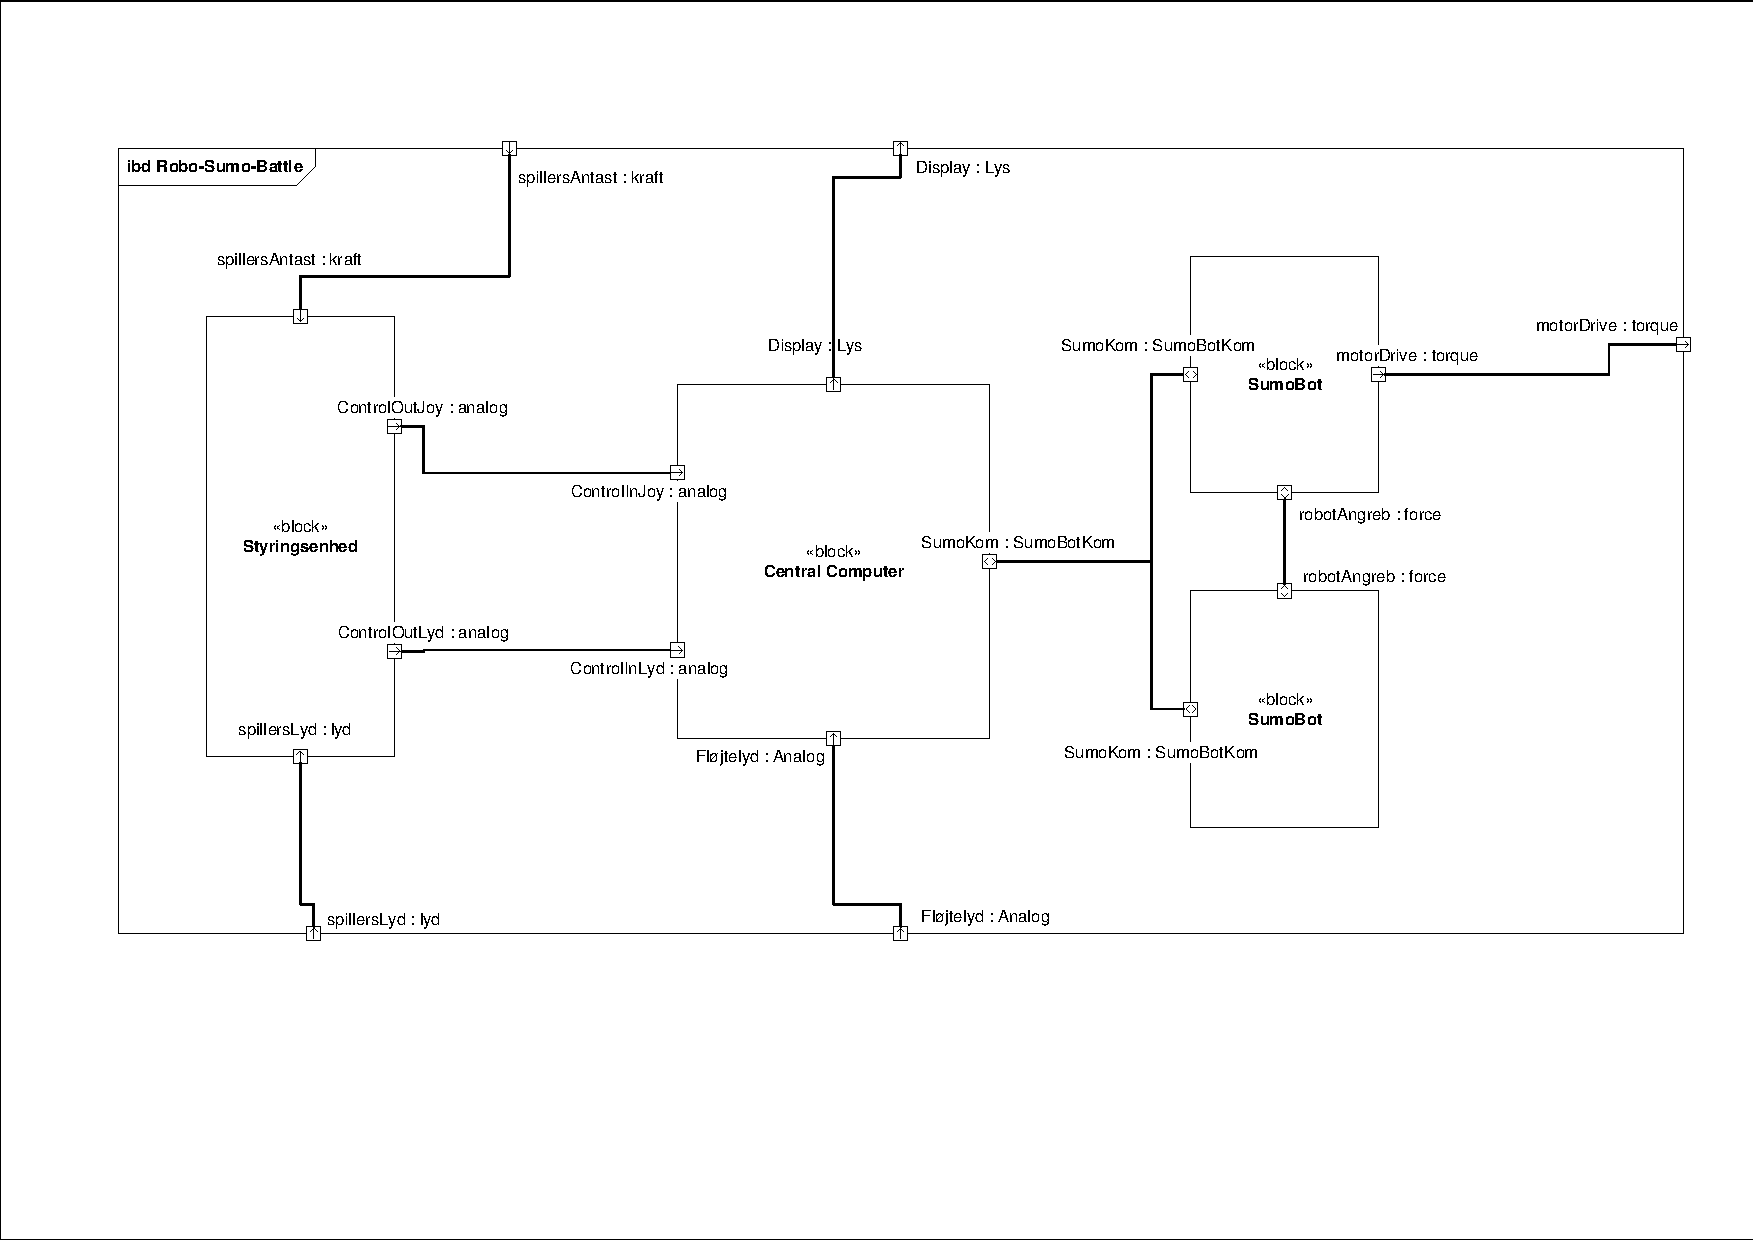
\includegraphics[page=1,width=1\linewidth]{figs/Diagrammer/IBD.pdf}
	\caption{System IBD}
	\label{fig:IBD_System_old}
\end{figure*}

\begin{figure*}[hpt]
	\centering
   	\includegraphics[page=3,width=1\linewidth]{figs/Diagrammer/IBD.pdf}
	\caption{IBD for Central Computer, se \tabref{interface_table_CentralComputer} for interfacebeskrivelse}
	\label{fig:IBD_CentralComputer}
\end{figure*}
\begin{figure*}[hpt]
	\centering
   	\includegraphics[page=2,width=1\linewidth]{figs/Diagrammer/IBD.pdf}
	\caption{IBD for Styringsenhed, se \tabref{interface_table_Styringsenhed} for interfacebeskrivelse}
	\label{fig:IBD_Styringsenhed}
\end{figure*}
\begin{figure*}[hpt]
	\centering
   	\includegraphics[page=4,width=1\linewidth]{figs/Diagrammer/IBD.pdf}
	\caption{IBD for SumoBot, se \tabref{interface_table_SumoBot} for interfacebeskrivelse}
	\label{fig:IBD_SumoBot}
\end{figure*}

\subsection{Interface beskrivelser}
Der er udarbejdet en interface beskrivelse for de mere komplekse interfaces. For \figref{IBD_SumoBot} findes en dertilhørende interfacebeskrivelse i  \tabref{interface_table_SumoBot}.

For \figref{IBD_CentralComputer} findes en dertilhørende interfacebeskrivelse i \tabref{interface_table_CentralComputer}.
%%%%%%%%%%%%%%%%%
% 2020/10/24 - Adam
% Jeg har tilladt mig at "rydde" op i koden her, ved at tage udgangspunkt i UseCase.sty - Der er lavet et nyt environment \begin{SignalDescrption}{Navn}{label}
% Her i kan \signalbeskrivelse{navn}{type}{beskrivelse} skrives. - Se Grp6_tabels for mere info.
% Dette skulle gerne sikret et ensartet udtryk, samt et enkelt workflow. 
%%%%%%%%%%%%%%%%%
\begin{SignalDescription}{Central Computer}{CentralComputer}
    \signalbeskrivelse{in ctrlInJoy       }{Digital     }{Seriel forbindelse med defineret retning og hastighed}
    \signalbeskrivelse{in ctrlInLyd       }{Digital     }{Seriel forbindelse med defineret retning og hastighed}
    \signalbeskrivelse{out DisplayDataOut }{Digital Bus }{6 parallelforbindelser der overføre displayinformation}
    \signalbeskrivelse{out LCDOut         }{Light       }{Spilinformation til brugerne.}
    \signalbeskrivelse{inout robotKom     }{WIFI        }{Trådløs tovejskommunikation, til styring af SumoBot  og returnering af attacks }
\end{SignalDescription}

\begin{SignalDescription}{Styringsenhed}{Styringsenhed}
    \signalbeskrivelse{in ctrlInLyd    }{analog              }{\tbr Et lydsignal med frekvensindhold 100-10000 Hz}
    \signalbeskrivelse{in filterIn     }{analog              }{\tbr Lydsignal fra blokfløjte, muligvis overlejret med støj }
    \signalbeskrivelse{out joyStickOut }{                    }{\textbf{Bus med 5 signaler}:}
    \signalbeskrivelse{                }{1: analogX          }{spænding variende mellem 0 og VCC}
    \signalbeskrivelse{                }{2: analogY          }{spænding variende mellem 0 og VCC}
    \signalbeskrivelse{                }{3: digital          }{switch til at trykke på joystick controller}
    \signalbeskrivelse{                }{4:  VCC             }{5V}
    \signalbeskrivelse{                }{5: GND              }{0V}
    \signalbeskrivelse{out Mikrofon    }{analog              }{Udgangsimpedans 2,2k Ohm \tbr                               }
    \signalbeskrivelse{                }{                    }{Udgangsspænding 6,3 mV/Pa/1 kHz \tbr                        }
    \signalbeskrivelse{out ctrlOutJoy  }{analog              }{\tbr Samme som joyStickOut? Tilpasset i amplitude?          }
    \signalbeskrivelse{out ctrlOutLyd  }{\tbr analog/digital }{\tbr Interface til central computer                         }
\end{SignalDescription}


\begin{SignalDescription}{SumoBot}{SumoBot}
\signalbeskrivelse{in/out SumoBotKom      }{SumoBotKom    }{WiFi\tbr signal fra Central Computer.    }
\signalbeskrivelse{in/out SumoBotCMD      }{SumoBotCMD    }{Signal til Microkontroller.              }
\signalbeskrivelse{in pakoersel           }{Force        }{ Fysisk påvirkning fra omverdenen.       }
\signalbeskrivelse{out pakoerselSignal    }{digital      }{ Logisk I/O signal.                      }
\signalbeskrivelse{pakoerselRegistrerin   }{Digital      }{ Logisk I/O signal.                      }
\signalbeskrivelse{out motorCmdOutLeft    }{Seriel        }{Signal til motorstyring om venstre motor.}
\signalbeskrivelse{out motorCmdOutRight   }{Seriel        }{Signal til motorstyring om højre motor.  }
\signalbeskrivelse{in motorCommandinLeft  }{Seriel        }{Signal til motorstyring om venstre motor.}
\signalbeskrivelse{in motorCommandInRight }{Seriel        }{Signal til motorstyring om højre motor.  }
\signalbeskrivelse{out motorCtrOut[2]     }{PWM           }{PWM signal til motor.                    }
\signalbeskrivelse{in motorCtrIn[2]       }{PWM           }{PWM signal til motor.                    }
\signalbeskrivelse{out motorTorqueOut     }{torque        }{Energi fra motor til hjul.               }
\signalbeskrivelse{in ChargePowerIn       }{DC            }{DC strøm fra oplader til batteri.        }
\signalbeskrivelse{in powerBat            }{DC            }{12V\tbr fra batteri.                     }
\signalbeskrivelse{in MCPower             }{DC            }{5V Forsyning.                            }
\signalbeskrivelse{out PowerOut           }{DC            }{5V forsyning.                            }
\end{SignalDescription}


% \begin{table*}[]
%     \centering
%     \caption{Interfacebeskrivelse for Central Computer}
%     \label{tab:interface_table_CentralComputer}
%     \begin{tabular}{lp{5cm}p{7cm}}\toprule
%         Navn              & Type       & Beskrivelse\\                                                                                                                                 
%         in ctrlInJoy        & Digital    & Seriel forbindelse med defineret retning og hastighed\\
%         in ctrlInLyd        & Digital    & Seriel forbindelse med defineret retning og hastighed\\     
%         out DisplayDataOut  & Digital Bus     & 6 parallelforbindelser der overføre displayinformation\\
%         out LCDOut                & Light    & Spilinformation til brugerne.\\
%         inout robotKom       & WIFI              & Trådløs tovejskommunikation, til styring af SumoBot  og returnering af attacks\\
%         \bottomrule
%     \end{tabular}%
% \end{table*}

% \begin{table*}[]
%     \centering
%     \caption{Interfacebeskrivelse for Styringsenhed}
%     \label{tab:interface_table_Styringsenhed}
%     \begin{tabular}{lp{5cm}p{7cm}}\toprule
%         Navn              & Type       & Beskrivelse\\                                                                                                                                 
%         in ctrlInLyd      & analog     & \tbr Et lydsignal med frekvensindhold 100-10000 Hz\\
%         in filterIn       & analog     & \tbr Lydsignal fra blokfløjte, muligvis overlejret med støj\\                                                                                             
%         out joyStickOut   &            & Bus med 5 signaler:\\
%                           & 1: analogX & spænding variende mellem 0 og VCC\\                                                                                                        
%                           & 2: analogY & spænding variende mellem 0 og VCC\\                                                                                                            
%                           & 3: digital & switch til at trykke på joystick controller\\                                                                                                                
%                           & 4:  VCC    & 5V                                         \\                                                                                                      
%                           & 5: GND     & 0V                                         \\
%         out Mikrofon      & analog     & Udgangsimpedans 2,2k Ohm \tbr\\
%                           &            & Udgangsspænding 6,3 mV/Pa/1 kHz \tbr\\
%         out ctrlOutJoy & analog & \tbr Samme som joyStickOut? Tilpasset i amplitude?\\
%         out ctrlOutLyd & \tbr analog/digital & \tbr Interface til central computer\\                                                                                               
%         \\
%                 \bottomrule
%     \end{tabular}%
% \end{table*}